\section{\label{sec:clas.st}Start Counter (\abbr{ST})}

The first incarnation of \abbr{CLAS} in 1996 had a three segment start counter, each covering two sectors. The data acquisition (\abbr{DAQ}) system at that time had a maximum rate of less than 1~kHz which limited the beam current the detector could handle. Therefore, the hit rate in the start counter was low and the triggering was efficient enough to allow only a few false events. As time went by, the \abbr{DAQ} became more efficient and by 2005 the maximum handling rate was $\sim5$~kHz. This rate was high enough to cause this start counter to act as an open gate in the trigger.

Youri Sharabian, a \abbr{JLab} staff scientist with Hall \desg{B}, designed and built a new 24-segment start counter\cite{clas.st} (\abbr{ST}) in 2006. It was first used with the \emph{g10} experiment\cite{clas.thesis.mckinnon} and it provided better timing and spatial resolution (see Sec.~\ref{sec:data.calib.systems}) as well as the ability to handle much higher beam currents.

The new start counter, shown in Fig.~\ref{fig:clas.st}, consists of 24 scintillation paddles which surrounds the 40~cm target hermetically within the acceptance of the drift-chambers. There are four paddles for each sector and two different paddle shapes. The start counter is capable of approximately 350~ps timing resolution making it useful to identify the hit in the tagger associated with the event. The segmentation allows for event rates that approach the tagger and \abbr{DAQ} limits.

\begin{figure}\begin{center}
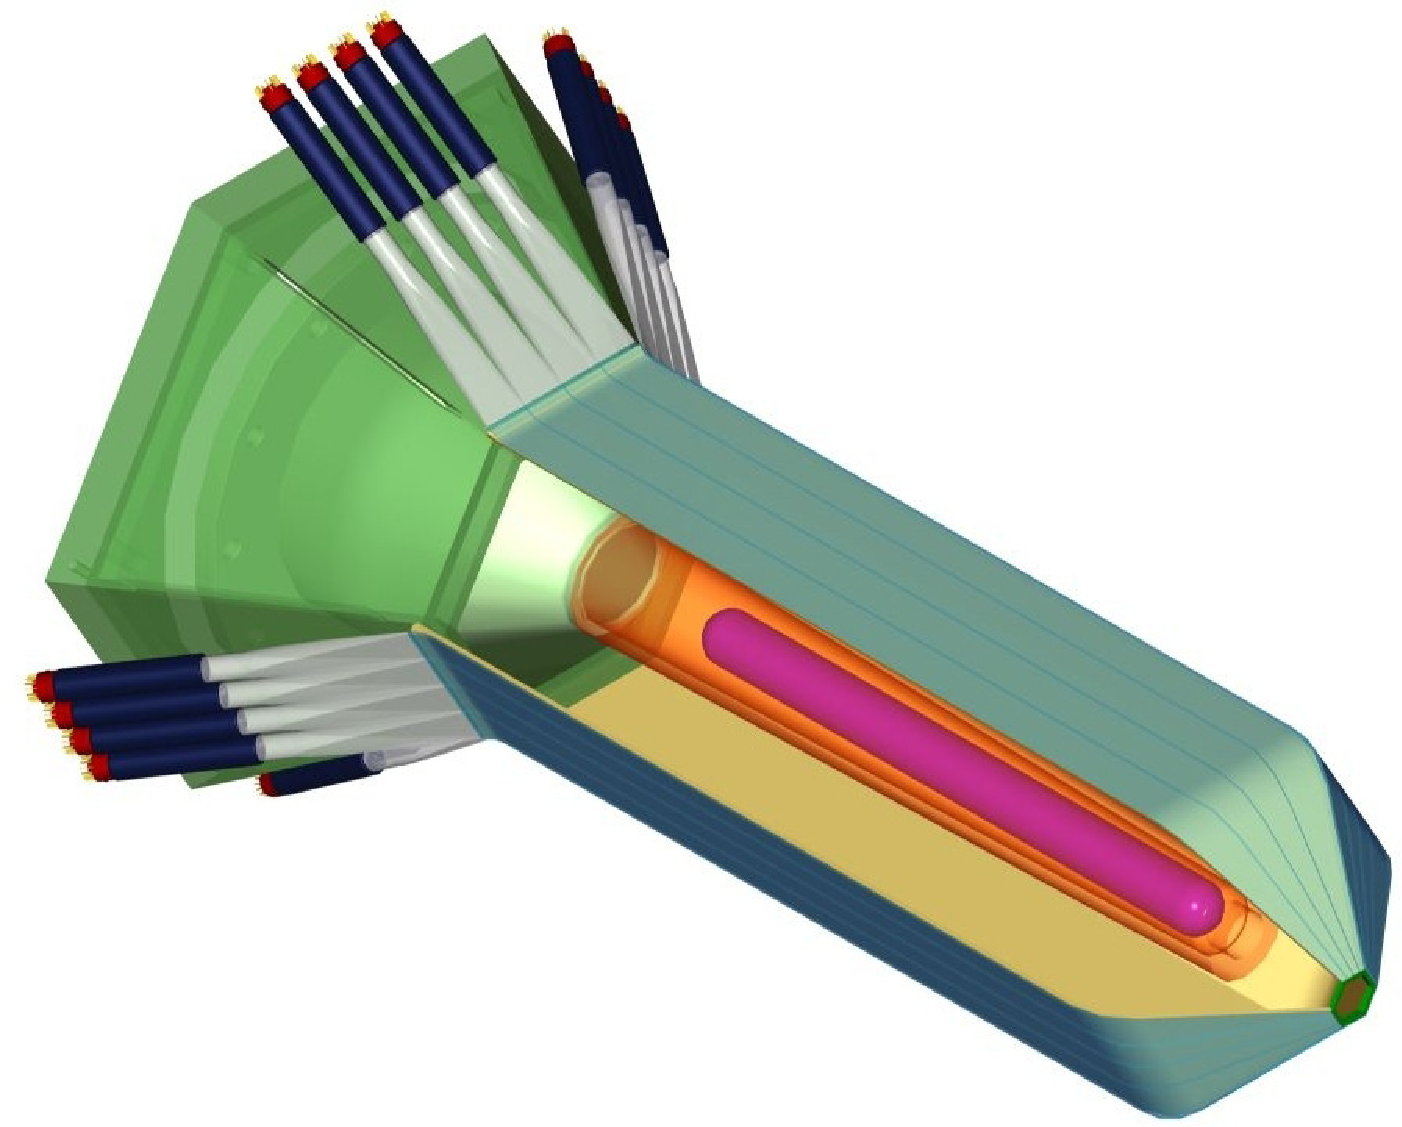
\includegraphics[width=0.8\figwidth]{\grpath/hall-b/start_counter.pdf}
\caption[Start Counter Schematic]{\label{fig:clas.st}{\coloronline}Schematic of the start counter (\abbr{ST}) with the 40~cm long target cell (purple) at the center. The beam enters from the upper left of the figure.}
\end{center}\end{figure}

\begin{figure}\begin{center}
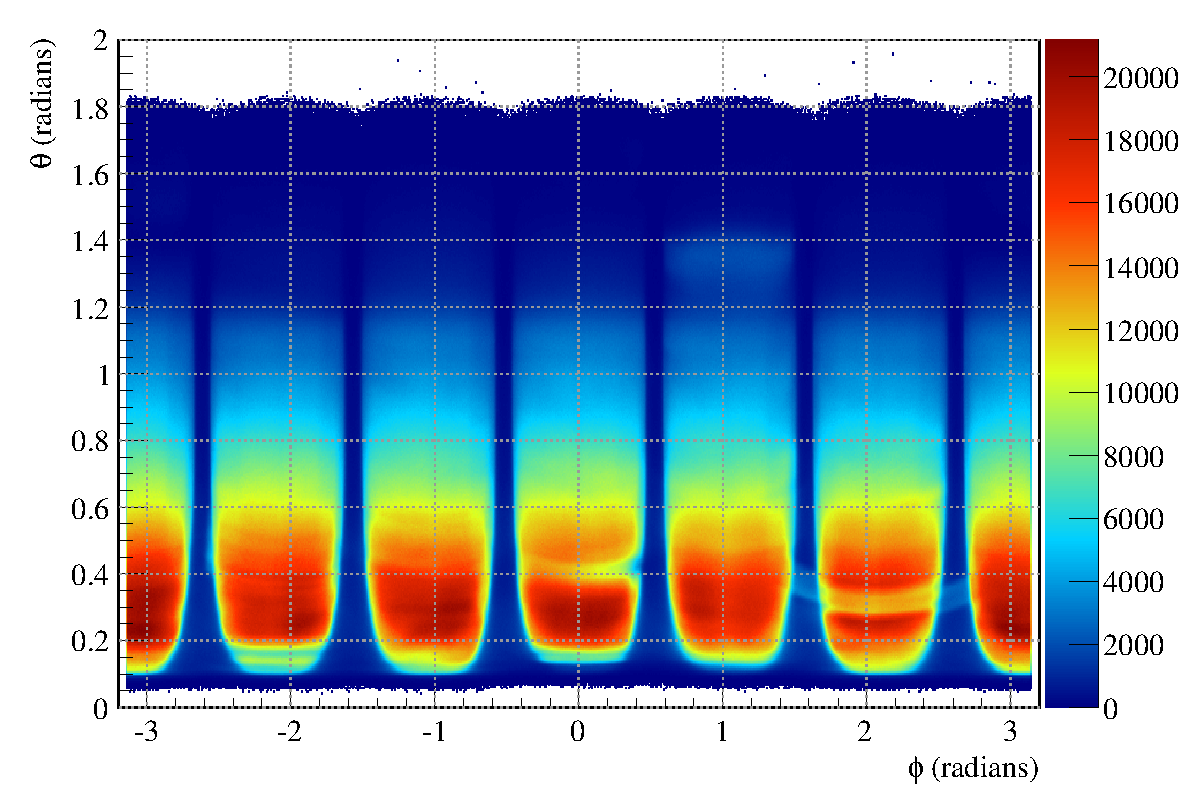
\includegraphics[width=\figwidth]{\grpath/reconstruction/coverage_st.pdf}
\caption[Start Counter Angular Coverage]{\label{fig:clas.st.coverage}{\coloronline}Angular coverage in the lab frame of the tracks that had an associated start counter hit showing that the \abbr{ST} covered the entire \abbr{DC}/\abbr{TOF} acceptance region which is shown in Fig.~\ref{fig:clas.tof.coverage}.}
\end{center}\end{figure}




%\begin{comment}
%
%\subsection{\label{sec:clas.st.eff}Efficiency Analysis}
%
%\todo{NOTE: I'm not sure if I want to keep this section. The numbers quoted are only from memory and are not reliable enough to put here at the moment.}
%
%About a year before \g12, we made some effort to understand the limiting factor on the \abbr{DAQ} rate for \abbr{CLAS}. At the time, it seemed that a start counter segmented in $\theta$ as well as $\phi$ might admit a higher beam current and therefore a higher physics event rate. Using phase-space Monte Carlo of three \emph{prong} events (p $\pi^+$ $\pi^-$) we were able to determine that two tracks will pass through the same \abbr{ST} paddle (in the current 24-paddle configuration) less than 5\% of the time. For topologies requiring four tracks, this increases to about 10\%. This only affects events on the trigger level, and since \g12 used a two-\emph{prong} trigger, the determination was that the 24-segment \abbr{ST} was sufficient. The tracks that use the same start counter hit in the data, since they enter the \abbr{ST} at about the same time, will not be lost during reconstruction.
%
%\begin{figure}\begin{center}
%%\includegraphics[width=0.8\figwidth]{\grpath/reconstruction/start_counter_eff.pdf}
%\caption[Start Counter Efficiency]{\label{fig:clas.st.eff}\todo{This plot must be recreated} Percentage of the track pairs that enter the same \abbr{ST} paddle for topologies increasing in number of particles. The trigger used for \g12 had a two-\emph{prong} configuration and therefore the number events lost at the trigger level was $<1\%$.}
%\end{center}\end{figure}
%
%\end{comment}
